
\chapter{Variabili Aleatorie Continue}
\section{Variabili Aleatorie Continue}

\subsection{Introduzione e intuizione}

In teoria della probabilità, una \textbf{variabile aleatoria}
è una funzione che associa un numero reale a ciascun possibile
esito di un esperimento casuale.

Le variabili aleatorie possono essere classificate, tra le altre,
in due categorie fondamentali:
\begin{itemize}
    \item \textbf{Variabili aleatorie discrete}: assumono valori
    in un insieme finito oppure numerabile.

    \item \textbf{Variabili aleatorie continue}: sono descritte
    da una funzione di densità e le probabilità sono calcolate
    integrando tale funzione su intervalli o, più in generale,
    su insiemi misurabili.
\end{itemize}

\paragraph{Perché sono necessarie le variabili aleatorie continue?}

Consideriamo un esperimento consistente nella misurazione
del tempo necessario a un computer per completare
un'operazione.

Indichiamo con $X$ tale tempo, espresso in secondi.

Potremmo osservare, ad esempio:
\[
X=1.2,\qquad X=1.25,\qquad X=1.2537.
\]

In un modello matematico idealizzato, il tempo può
assumere qualsiasi valore reale non negativo.

Pertanto, non è conveniente descrivere il fenomeno
assegnando una probabilità a ogni singolo valore.

Risulta invece naturale porre domande come:
\begin{itemize}
    \item Qual è la probabilità che l'operazione
    termini entro 2 secondi?

    \item Qual è la probabilità che richieda
    tra 1 e 3 secondi?

    \item Qual è il tempo medio di esecuzione?
\end{itemize}

Le variabili aleatorie continue permettono di rispondere
a queste domande attraverso una
\textbf{funzione di densità di probabilità}.

\begin{example}{Tempo di risposta}
Supponiamo che $X$ rappresenti il tempo di risposta
di un server.

L'evento
\[
\{1\leq X\leq 2\}
\]
indica che il server risponde in un tempo
compreso tra 1 e 2 secondi.

Il nostro interesse non consiste nel determinare
la probabilità di un tempo esattamente pari
a $1.473829$ secondi, ma quella di osservare
un tempo appartenente a un certo intervallo.
\end{example}


\subsection{Definizione formale}

Prima di definire una variabile aleatoria continua,
richiamiamo la definizione generale di variabile aleatoria.

\begin{definition}{Variabile aleatoria}
Dato uno spazio di probabilità
\[
(\Omega,\mathcal{F},P),
\]
una variabile aleatoria reale è una funzione misurabile
\[
X:\Omega\longrightarrow\mathbb{R}.
\]

Essa associa a ogni esito $\omega\in\Omega$
un numero reale $X(\omega)$.

La misurabilità garantisce che eventi come
\[
\{\omega\in\Omega:X(\omega)\leq x\}
\]
appartengano a $\mathcal{F}$ e abbiano quindi
una probabilità ben definita.
\end{definition}

\begin{definition}{Variabile aleatoria continua}
Una variabile aleatoria reale $X$ si dice
\textbf{assolutamente continua}, o continua nel senso
delle distribuzioni con densità, se esiste
una funzione
\[
f_X:\mathbb{R}\longrightarrow[0,+\infty)
\]
tale che, per ogni insieme boreliano
$A\subseteq\mathbb{R}$,
\[
\boxed{
P(X\in A)=\int_A f_X(x)\,dx.
}
\]

La funzione $f_X$ prende il nome di
\textbf{funzione di densità di probabilità},
o \textbf{Probability Density Function (PDF)}.
\end{definition}

\paragraph{Osservazione terminologica}

Nel linguaggio introduttivo, le distribuzioni
che ammettono una densità vengono generalmente
chiamate distribuzioni continue.

In termini matematici, tuttavia,
una funzione di ripartizione continua
non garantisce necessariamente l'esistenza
di una densità.

In questi appunti, con variabile aleatoria
continua intenderemo una variabile aleatoria
\textbf{assolutamente continua}.

\subsection{Funzione di densità di probabilità}

La funzione di densità $f_X(x)$ descrive
come la probabilità è distribuita
lungo la retta reale.

È importante distinguere:
\begin{itemize}
    \item $f_X(x)$: densità di probabilità
    nel punto $x$;
    \item $P(a\leq X\leq b)$: probabilità
    che $X$ appartenga all'intervallo $[a,b]$.
\end{itemize}

Il valore $f_X(x)$ non rappresenta,
in generale, una probabilità.

La probabilità viene ottenuta
calcolando un'area sotto la curva della densità.

\[
\boxed{
P(a\leq X\leq b)
=
\int_a^b f_X(x)\,dx.
}
\]

\subsubsection{Proprietà fondamentali della densità}

Una funzione $f_X$ è una densità di probabilità
se soddisfa due proprietà fondamentali.

\paragraph{1. Non negatività}

\[
\boxed{
f_X(x)\geq 0
\qquad \forall x\in\mathbb{R}.
}
\]

La densità non può essere negativa,
poiché l'integrale su qualsiasi insieme
deve rappresentare una probabilità
non negativa.

\paragraph{2. Normalizzazione}

\[
\boxed{
\int_{-\infty}^{+\infty}
f_X(x)\,dx=1.
}
\]

L'area totale sotto la curva deve essere 1.

Questo deriva dal fatto che
\[
P(X\in\mathbb{R})=1.
\]

\paragraph{3. La densità può essere maggiore di 1}

Non è necessario che
\[
f_X(x)\leq 1.
\]

Infatti, $f_X(x)$ non rappresenta
una probabilità puntuale.

Per esempio, la funzione
\[
f_X(x)=
\begin{cases}
2 & 0\leq x\leq \frac12,\\
0 & \text{altrimenti}
\end{cases}
\]
è una densità valida, perché
\[
\int_0^{1/2}2\,dx=1.
\]

\subsubsection{Interpretazione geometrica della probabilità}

Il seguente grafico mostra una densità normale
e l'area corrispondente alla probabilità
che $X$ sia compresa tra $-1$ e $1$.

\begin{center}
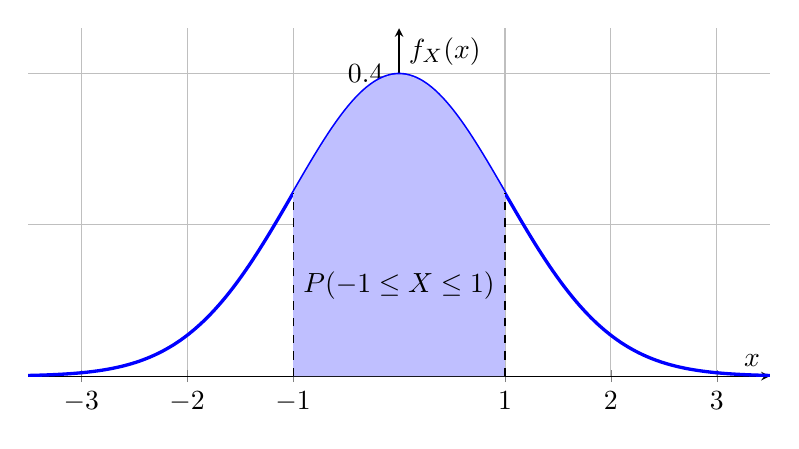
\begin{tikzpicture}
\begin{axis}[
    width=11cm,
    height=6cm,
    axis lines=middle,
    xlabel={$x$},
    ylabel={$f_X(x)$},
    xmin=-3.5,
    xmax=3.5,
    ymin=0,
    ymax=0.46,
    samples=200,
    domain=-3.5:3.5,
    grid=major
]
\addplot[
    blue,
    very thick
]
{exp(-x^2/2)/sqrt(2*pi)};

\addplot[
    blue!25,
    draw=none,
    fill=blue!25,
    domain=-1:1
]
{exp(-x^2/2)/sqrt(2*pi)}
\closedcycle;

\draw[dashed] (axis cs:-1,0)--(axis cs:-1,0.242);
\draw[dashed] (axis cs:1,0)--(axis cs:1,0.242);

\node at (axis cs:0,0.12)
{$P(-1\leq X\leq1)$};

\end{axis}
\end{tikzpicture}
\end{center}

L'area evidenziata rappresenta
\[
P(-1\leq X\leq 1)
=
\int_{-1}^{1}f_X(x)\,dx.
\]

\subsection{Probabilità di un singolo valore}

Una delle differenze più importanti
tra una variabile aleatoria discreta
e una assolutamente continua
riguarda la probabilità dei singoli valori.

\begin{theorem}
Se $X$ è una variabile aleatoria
assolutamente continua, allora
per ogni $a\in\mathbb{R}$:
\[
\boxed{P(X=a)=0.}
\]
\end{theorem}

\paragraph{Dimostrazione}

Per definizione,
\[
P(X=a)
=
\int_{\{a\}} f_X(x)\,dx.
\]

Poiché un singolo punto ha misura
di Lebesgue nulla, otteniamo
\[
P(X=a)=0.
\]

\paragraph{Interpretazione}

Questo non significa che il valore $a$
sia impossibile da osservare.

Significa che, nel modello continuo,
la probabilità associata a un singolo
valore esatto è nulla.

Per esempio:
\[
P(X=1.5)=0,
\]
ma può essere
\[
P(1.4\leq X\leq1.6)>0.
\]

\subsubsection{Conseguenza sugli intervalli}

Poiché i singoli punti hanno probabilità
nulla, si ha:
\[
\boxed{
P(a<X<b)
=
P(a\leq X<b)
=
P(a<X\leq b)
=
P(a\leq X\leq b).
}
\]

Quindi, per variabili aleatorie continue,
gli estremi aperti o chiusi
non modificano la probabilità.

\subsection{Funzione di ripartizione}

La funzione di ripartizione rappresenta
uno degli strumenti fondamentali
per descrivere qualsiasi variabile aleatoria.

\begin{definition}{Funzione di ripartizione}
La funzione di ripartizione,
o \textbf{Cumulative Distribution Function (CDF)},
di una variabile aleatoria $X$ è
\[
\boxed{
F_X(x)=P(X\leq x).
}
\]
\end{definition}

La funzione $F_X(x)$ descrive quindi
la probabilità accumulata fino al valore $x$.

\subsubsection{Relazione tra PDF e CDF}

Per una variabile aleatoria
assolutamente continua:
\[
\boxed{
F_X(x)
=
\int_{-\infty}^{x}
f_X(t)\,dt.
}
\]

Il simbolo $t$ è una variabile
di integrazione.

La formula significa che
per ottenere la probabilità
$P(X\leq x)$ dobbiamo sommare,
mediante integrazione,
la densità da $-\infty$ fino a $x$.

Viceversa, dove la funzione
di ripartizione è derivabile:
\[
\boxed{
f_X(x)=\frac{d}{dx}F_X(x).
}
\]

Più precisamente, per una distribuzione
assolutamente continua questa relazione
vale quasi ovunque.

\subsubsection{Proprietà della funzione di ripartizione}

La funzione $F_X$ soddisfa:

\begin{enumerate}
    \item \textbf{Limitatezza}
    \[
    0\leq F_X(x)\leq1.
    \]

    \item \textbf{Monotonia}
    \[
    x_1<x_2
    \implies
    F_X(x_1)\leq F_X(x_2).
    \]

    \item \textbf{Limiti agli estremi}
    \[
    \lim_{x\to-\infty}F_X(x)=0,
    \]
    \[
    \lim_{x\to+\infty}F_X(x)=1.
    \]

    \item \textbf{Continuità}

    Per una variabile aleatoria
    assolutamente continua,
    $F_X$ è continua su $\mathbb{R}$.
\end{enumerate}

\subsubsection{Calcolare le probabilità mediante la CDF}

Per $a<b$:
\[
\boxed{
P(a<X\leq b)=F_X(b)-F_X(a).
}
\]

Nel caso continuo, possiamo anche scrivere
\[
P(a\leq X\leq b)=F_X(b)-F_X(a).
\]

Inoltre:
\[
P(X>x)=1-F_X(x).
\]

\begin{example}{Calcolo della PDF e della CDF}

Consideriamo la densità
\[
f_X(x)=
\begin{cases}
2x & 0\leq x\leq1,\\
0 & \text{altrimenti}.
\end{cases}
\]

\textbf{Passo 1: verifica della normalizzazione.}

\[
\int_0^1 2x\,dx
=
[x^2]_0^1
=
1.
\]

La funzione è una densità valida.

\textbf{Passo 2: calcolo della CDF.}

Per $x<0$:
\[
F_X(x)=0.
\]

Per $0\leq x\leq1$:
\[
F_X(x)
=
\int_0^x 2t\,dt
=
[t^2]_0^x
=
x^2.
\]

Per $x>1$:
\[
F_X(x)=1.
\]

Pertanto:
\[
\boxed{
F_X(x)=
\begin{cases}
0 & x<0,\\
x^2 & 0\leq x\leq1,\\
1 & x>1.
\end{cases}
}
\]

\textbf{Passo 3: calcolo di una probabilità.}

Vogliamo determinare:
\[
P\left(\frac12\leq X\leq1\right).
\]

Utilizzando la CDF:
\[
P\left(\frac12\leq X\leq1\right)
=
F_X(1)-F_X\left(\frac12\right).
\]

Quindi:
\[
=1-\frac14
=\boxed{\frac34}.
\]

Lo stesso risultato si ottiene
integrando la densità:
\[
\int_{1/2}^1 2x\,dx
=
\frac34.
\]
\end{example}

\subsection{Supporto di una distribuzione}

\begin{definition}{Supporto}
Il supporto di una distribuzione è,
in termini rigorosi, il più piccolo
insieme chiuso avente probabilità 1.

Equivalentemente, è l'insieme dei punti
i cui ogni intorno aperto ha
probabilità positiva.
\end{definition}

Nel caso di una densità continua $f_X$,
il supporto coincide con la chiusura
dell'insieme
\[
\{x\in\mathbb{R}:f_X(x)>0\}.
\]

\begin{example}{Supporto di una densità uniforme}

Se
\[
f_X(x)=
\begin{cases}
\frac14 & 2\leq x\leq6,\\
0 & \text{altrove},
\end{cases}
\]
il supporto è
\[
\operatorname{supp}(X)=[2,6].
\]

Ciò significa che $X$ appartiene
all'intervallo $[2,6]$ con probabilità 1.
\end{example}


\section{Valore Atteso, Varianza e Momenti}

\subsection{Valore atteso}

Il valore atteso, chiamato anche
\textbf{media teorica}, descrive
la posizione centrale di una distribuzione.

Intuitivamente rappresenta
il valore medio che si otterrebbe
ripetendo l'esperimento casuale
molte volte e calcolando
la media dei risultati, sotto
le opportune condizioni.

\begin{definition}{Valore atteso}
Sia $X$ una variabile aleatoria
assolutamente continua con densità $f_X$.

Se
\[
\int_{-\infty}^{+\infty}
|x|f_X(x)\,dx<+\infty,
\]
il valore atteso di $X$ è
\[
\boxed{
\mathbb{E}[X]
=
\int_{-\infty}^{+\infty}
x f_X(x)\,dx.
}
\]

Viene comunemente indicato anche con
\[
\mu=\mathbb{E}[X].
\]
\end{definition}

\paragraph{Interpretazione della formula}

La formula
\[
\mathbb{E}[X]
=
\int_{-\infty}^{+\infty}
x f_X(x)\,dx
\]
può essere interpretata come
una media pesata.

Ogni valore $x$ contribuisce alla media
in funzione della densità di probabilità
presente nella sua regione.

Questo è l'analogo continuo
della formula discreta:
\[
\mathbb{E}[X]
=
\sum_x xP(X=x).
\]

\begin{example}{Media di una variabile uniforme}

Supponiamo che $X$ sia distribuita
uniformemente su $[0,4]$.

La densità è:
\[
f_X(x)=
\begin{cases}
\frac14 & 0\leq x\leq4,\\
0 & \text{altrimenti}.
\end{cases}
\]

Calcoliamo il valore atteso:
\[
\mathbb{E}[X]
=
\int_0^4 x\frac14\,dx.
\]

Portando fuori la costante:
\[
=
\frac14\int_0^4 x\,dx.
\]

Integrando:
\[
=
\frac14
\left[\frac{x^2}{2}\right]_0^4.
\]

Pertanto:
\[
=
\frac14\cdot\frac{16}{2}
=
\boxed{2}.
\]

Il valore medio è esattamente
il punto centrale dell'intervallo.
\end{example}

\subsubsection{Proprietà del valore atteso}

\paragraph{Linearità}

Per costanti $a,b\in\mathbb{R}$:
\[
\boxed{
\mathbb{E}[aX+b]
=
a\mathbb{E}[X]+b.
}
\]

Più in generale, se i valori attesi esistono:
\[
\boxed{
\mathbb{E}[aX+bY]
=
a\mathbb{E}[X]+b\mathbb{E}[Y].
}
\]

Non è necessario che $X$ e $Y$
siano indipendenti.

\paragraph{Valore atteso di una costante}

\[
\mathbb{E}[c]=c.
\]

\paragraph{Valore atteso di una funzione}

\begin{theorem}{Legge dello statistico inconsapevole}
Sia $g:\mathbb{R}\to\mathbb{R}$
una funzione misurabile.

Se $g(X)$ è integrabile:
\[
\boxed{
\mathbb{E}[g(X)]
=
\int_{-\infty}^{+\infty}
g(x)f_X(x)\,dx.
}
\]
\end{theorem}

Questa formula consente di calcolare
il valore atteso di una trasformazione
senza dover determinare preliminarmente
la densità della nuova variabile aleatoria.

\begin{example}{Valore atteso del quadrato}

Sia
\[
f_X(x)=
\begin{cases}
2x & 0\leq x\leq1,\\
0 & \text{altrove}.
\end{cases}
\]

Vogliamo calcolare
\[
\mathbb{E}[X^2].
\]

Applicando la formula:
\[
\mathbb{E}[X^2]
=
\int_0^1 x^2(2x)\,dx.
\]

Quindi:
\[
=
2\int_0^1 x^3\,dx
=
2\left[\frac{x^4}{4}\right]_0^1
=
\boxed{\frac12}.
\]
\end{example}


\subsection{Varianza}

Il valore atteso ci informa
sulla posizione centrale,
ma non descrive quanto
i possibili valori siano dispersi.

Due variabili aleatorie possono
avere lo stesso valore atteso,
pur presentando distribuzioni
molto differenti.

Per misurare la dispersione
introduciamo la varianza.

\begin{definition}{Varianza}
Sia $X$ una variabile aleatoria
con valore atteso finito
\[
\mu=\mathbb{E}[X].
\]

Se esiste il secondo momento,
la varianza è definita come
\[
\boxed{
\operatorname{Var}(X)
=
\mathbb{E}[(X-\mu)^2].
}
\]

Nel caso assolutamente continuo:
\[
\boxed{
\operatorname{Var}(X)
=
\int_{-\infty}^{+\infty}
(x-\mu)^2f_X(x)\,dx.
}
\]
\end{definition}

\paragraph{Interpretazione}

La quantità
\[
X-\mu
\]
misura quanto una realizzazione
si discosta dalla media.

Elevandola al quadrato:
\[
(X-\mu)^2,
\]
si ottengono contributi non negativi
e si attribuisce maggiore peso
agli scostamenti più grandi.

La varianza è il valore atteso
di questi scostamenti quadratici.

\subsubsection{Formula alternativa della varianza}

Partiamo dalla definizione:
\[
\operatorname{Var}(X)
=
\mathbb{E}[(X-\mu)^2].
\]

Sviluppiamo il quadrato:
\[
(X-\mu)^2
=
X^2-2\mu X+\mu^2.
\]

Applicando la linearità:
\[
\operatorname{Var}(X)
=
\mathbb{E}[X^2]
-2\mu\mathbb{E}[X]
+\mu^2.
\]

Poiché
\[
\mathbb{E}[X]=\mu,
\]
otteniamo
\[
=
\mathbb{E}[X^2]-2\mu^2+\mu^2.
\]

Quindi:
\[
\boxed{
\operatorname{Var}(X)
=
\mathbb{E}[X^2]
-
(\mathbb{E}[X])^2.
}
\]

Questa formula è spesso
più semplice da utilizzare
nei calcoli.

\begin{example}{Calcolo completo della varianza}

Consideriamo nuovamente:
\[
f_X(x)=
\begin{cases}
2x & 0\leq x\leq1,\\
0 & \text{altrove}.
\end{cases}
\]

\textbf{Passo 1: calcolo della media.}

\[
\mathbb{E}[X]
=
\int_0^1 x(2x)\,dx.
\]

\[
=
2\int_0^1 x^2\,dx
=
2\left[\frac{x^3}{3}\right]_0^1.
\]

Quindi:
\[
\mathbb{E}[X]=\frac23.
\]

\textbf{Passo 2: secondo momento.}

Abbiamo:
\[
\mathbb{E}[X^2]=\frac12.
\]

\textbf{Passo 3: formula alternativa.}

\[
\operatorname{Var}(X)
=
\frac12-\left(\frac23\right)^2.
\]

\[
=
\frac12-\frac49.
\]

Portando a denominatore comune:
\[
=
\frac9{18}-\frac8{18}.
\]

Pertanto:
\[
\boxed{
\operatorname{Var}(X)=\frac1{18}.
}
\]
\end{example}

\subsubsection{Proprietà della varianza}

\paragraph{Non negatività}
\[
\boxed{
\operatorname{Var}(X)\geq0.
}
\]

Questo perché
\[
(X-\mu)^2\geq0.
\]

\paragraph{Varianza di una costante}
\[
\operatorname{Var}(c)=0.
\]

\paragraph{Trasformazione affine}
\[
\boxed{
\operatorname{Var}(aX+b)
=
a^2\operatorname{Var}(X).
}
\]

Aggiungere una costante
non modifica la dispersione;
moltiplicare per $a$
moltiplica la varianza per $a^2$.

\paragraph{Varianza della somma}

Per due variabili con varianza finita:
\[
\boxed{
\operatorname{Var}(X+Y)
=
\operatorname{Var}(X)
+
\operatorname{Var}(Y)
+
2\operatorname{Cov}(X,Y).
}
\]

Se $X$ e $Y$ sono indipendenti,
la loro covarianza è zero,
quindi:
\[
\operatorname{Var}(X+Y)
=
\operatorname{Var}(X)
+
\operatorname{Var}(Y).
\]

\subsection{Deviazione standard}

\begin{definition}{Deviazione standard}
La deviazione standard
è la radice quadrata
della varianza:
\[
\boxed{
\sigma_X
=
\sqrt{\operatorname{Var}(X)}.
}
\]
\end{definition}

La varianza è espressa nel quadrato
dell'unità di misura originale.

La deviazione standard,
invece, ha la stessa
unità di misura di $X$.

\begin{example}{Tempo di esecuzione}

Supponiamo che
\[
\mathbb{E}[X]=5\text{ s}
\]
e
\[
\operatorname{Var}(X)=4\text{ s}^2.
\]

La deviazione standard è:
\[
\sigma_X=\sqrt4=2\text{ s}.
\]

Questo valore descrive una scala
tipica degli scostamenti dalla media.

Non significa che ogni osservazione
si discosti dalla media
esattamente di 2 secondi.
\end{example}

\subsection{Momenti di una variabile aleatoria}

\begin{definition}{Momento di ordine $k$}
Il momento rispetto all'origine
di ordine $k$ è
\[
\boxed{
m_k=\mathbb{E}[X^k]
=
\int_{-\infty}^{+\infty}
x^k f_X(x)\,dx,
}
\]
quando l'integrale esiste.
\end{definition}

In particolare:
\[
m_1=\mathbb{E}[X]
\]
è la media, mentre
\[
m_2=\mathbb{E}[X^2]
\]
è il secondo momento.

\begin{definition}{Momento centrale}
Il momento centrale di ordine $k$ è
\[
\boxed{
\mu_k=\mathbb{E}[(X-\mu)^k].
}
\]
\end{definition}

Il secondo momento centrale coincide
con la varianza:
\[
\mu_2=\operatorname{Var}(X).
\]

Per distribuzioni con momenti adeguati
si definiscono anche:

\paragraph{Asimmetria}
\[
\gamma_1
=
\frac{\mathbb{E}[(X-\mu)^3]}{\sigma^3}.
\]

Un valore positivo indica
una maggiore estensione
della coda verso destra;
un valore negativo
indica una maggiore estensione
verso sinistra.

\paragraph{Curtosi}
\[
\beta_2
=
\frac{\mathbb{E}[(X-\mu)^4]}{\sigma^4}.
\]

È una misura sensibile
alla presenza di valori molto lontani
dalla media e alla struttura delle code.

L'eccesso di curtosi è
\[
\gamma_2=\beta_2-3,
\]
poiché una distribuzione normale
ha curtosi uguale a 3.


\section{Quantili, Mediana e Moda}

\subsection{Quantili}

\begin{definition}{Quantile}
Dato $p\in(0,1)$, il quantile
di ordine $p$ è
\[
\boxed{
q_p=\inf\{x\in\mathbb{R}:F_X(x)\geq p\}.
}
\]

Se la CDF è continua
e strettamente crescente
nella regione considerata,
esso soddisfa
\[
F_X(q_p)=p.
\]
\end{definition}

\begin{example}{Interpretazione dei quantili}

Il quantile di ordine $0.90$
è una soglia tale che,
nel caso continuo,
\[
P(X\leq q_{0.90})=0.90.
\]

Pertanto il 90\% della probabilità
si trova a sinistra di tale soglia,
e il restante 10\% a destra.
\end{example}

\subsection{Mediana}

\begin{definition}{Mediana}
Una mediana $m$ è un valore tale che
\[
P(X\leq m)\geq\frac12
\]
e
\[
P(X\geq m)\geq\frac12.
\]

Per una distribuzione continua,
un quantile di ordine $0.5$
è una mediana.
\end{definition}

\subsection{Moda}

\begin{definition}{Moda}
Una moda di una distribuzione
con densità $f_X$ è un punto
$x_{\mathrm{moda}}$
nel quale la densità raggiunge
il proprio massimo globale,
quando tale massimo esiste:
\[
f_X(x_{\mathrm{moda}})
=
\max_x f_X(x).
\]
\end{definition}

\paragraph{Differenza tra media, mediana e moda}

\begin{itemize}
    \item La \textbf{media} è il valore atteso.
    \item La \textbf{mediana} divide
    la probabilità in due parti
    di almeno il 50\%.
    \item La \textbf{moda} identifica
    un punto di massima densità.
\end{itemize}

Questi tre valori possono coincidere
oppure essere differenti,
a seconda della distribuzione.


\section{Principali Distribuzioni Continue}

\subsection{Distribuzione uniforme continua}

\subsubsection{Idea intuitiva}

La distribuzione uniforme continua
modella situazioni in cui
intervalli della stessa lunghezza,
contenuti nel supporto,
hanno la stessa probabilità.

Si tratta di un modello adatto
quando non esistono regioni
dell'intervallo favorite rispetto ad altre.

\begin{example}{Numero casuale uniforme}

Un generatore produce un numero reale
casuale tra 0 e 1.

Se la generazione è uniforme,
qualsiasi intervallo di lunghezza $0.1$
ha probabilità $0.1$.

Ad esempio:
\[
P(0.2\leq X\leq0.3)=0.1,
\]
e
\[
P(0.7\leq X\leq0.8)=0.1.
\]
\end{example}

\begin{definition}{Distribuzione uniforme}
Una variabile aleatoria $X$ segue
una distribuzione uniforme
nell'intervallo $[a,b]$, con $a<b$,
se la sua densità è:
\[
\boxed{
f_X(x)=
\begin{cases}
\frac1{b-a} & a\leq x\leq b,\\
0 & \text{altrimenti}.
\end{cases}
}
\]

Si scrive
\[
X\sim\mathcal{U}(a,b).
\]
\end{definition}

\subsubsection{Verifica della densità}

\[
\int_a^b\frac1{b-a}\,dx
=
\frac1{b-a}[x]_a^b
=
1.
\]

\subsubsection{Funzione di ripartizione}

\[
\boxed{
F_X(x)=
\begin{cases}
0 & x<a,\\
\frac{x-a}{b-a} & a\leq x\leq b,\\
1 & x>b.
\end{cases}
}
\]

\subsubsection{Media e varianza}

\[
\boxed{
\mathbb{E}[X]=\frac{a+b}{2}.
}
\]

\[
\boxed{
\operatorname{Var}(X)=\frac{(b-a)^2}{12}.
}
\]

\subsubsection{Grafico della densità}

\begin{center}
\begin{tikzpicture}
\begin{axis}[
    width=10cm,
    height=5cm,
    xmin=-0.5,
    xmax=5.5,
    ymin=0,
    ymax=0.5,
    axis lines=middle,
    xlabel={$x$},
    ylabel={$f_X(x)$},
    xtick={0,1,4,5},
    ytick={0.3333},
    yticklabels={$\frac13$}
]
\addplot[blue,very thick]
coordinates {(-0.5,0) (1,0)};
\addplot[blue,very thick]
coordinates {(1,0.3333) (4,0.3333)};
\addplot[blue,very thick]
coordinates {(4,0) (5.5,0)};
\addplot[dashed]
coordinates {(1,0) (1,0.3333)};
\addplot[dashed]
coordinates {(4,0) (4,0.3333)};
\end{axis}
\end{tikzpicture}
\end{center}

Il grafico rappresenta
\[
X\sim\mathcal{U}(1,4).
\]

\begin{example}{Calcolo di una probabilità}

Sia
\[
X\sim\mathcal{U}(2,10).
\]

Calcoliamo
\[
P(4\leq X\leq7).
\]

La densità è
\[
f_X(x)=\frac18
\qquad 2\leq x\leq10.
\]

Pertanto:
\[
P(4\leq X\leq7)
=
\int_4^7\frac18\,dx.
\]

\[
=
\frac{7-4}{8}
=
\boxed{\frac38}.
\]

La probabilità è il rapporto
tra la lunghezza dell'intervallo
richiesto e la lunghezza
dell'intero supporto.
\end{example}


\subsection{Distribuzione esponenziale}

\subsubsection{Idea intuitiva}

La distribuzione esponenziale
viene utilizzata per modellare
i tempi di attesa tra eventi
che si verificano secondo
un processo di Poisson omogeneo.

Esempi:
\begin{itemize}
    \item Tempo tra due richieste
    consecutive a un server.
    \item Tempo tra due chiamate
    consecutive a un centralino.
    \item Durata di funzionamento
    di un componente con tasso
    di guasto costante.
\end{itemize}

Questi impieghi sono appropriati
quando le ipotesi del modello,
in particolare il tasso costante,
sono ragionevoli.

\begin{definition}{Distribuzione esponenziale}
Una variabile aleatoria $X$
segue una distribuzione esponenziale
di parametro $\lambda>0$ se
\[
\boxed{
f_X(x)=
\begin{cases}
\lambda e^{-\lambda x} & x\geq0,\\
0 & x<0.
\end{cases}
}
\]

Si scrive
\[
X\sim\operatorname{Exp}(\lambda).
\]

Il parametro $\lambda$ rappresenta
un tasso per unità di tempo.
\end{definition}

\subsubsection{Funzione di ripartizione}

Per $x\geq0$:
\[
F_X(x)
=
\int_0^x\lambda e^{-\lambda t}\,dt.
\]

Integrando:
\[
F_X(x)
=
[-e^{-\lambda t}]_0^x.
\]

Quindi:
\[
\boxed{
F_X(x)=
\begin{cases}
0 & x<0,\\
1-e^{-\lambda x} & x\geq0.
\end{cases}
}
\]

In particolare:
\[
\boxed{
P(X>x)=e^{-\lambda x}.
}
\]

\subsubsection{Media e varianza}

\[
\boxed{
\mathbb{E}[X]=\frac1\lambda.
}
\]

\[
\boxed{
\operatorname{Var}(X)=\frac1{\lambda^2}.
}
\]

La deviazione standard è
\[
\sigma_X=\frac1\lambda.
\]

\subsubsection{Proprietà di assenza di memoria}

La distribuzione esponenziale
gode della proprietà
\textbf{memoryless}:

\[
\boxed{
P(X>s+t\mid X>s)=P(X>t)
}
\]
per ogni $s,t\geq0$.

\paragraph{Interpretazione}

Supponiamo che $X$ rappresenti
il tempo di attesa prima
dell'arrivo della prossima richiesta.

Se abbiamo già atteso $s$ secondi
senza osservare richieste,
la distribuzione del tempo
di attesa residuo
non dipende dal tempo già trascorso.

\subsubsection{Grafico}

\begin{center}
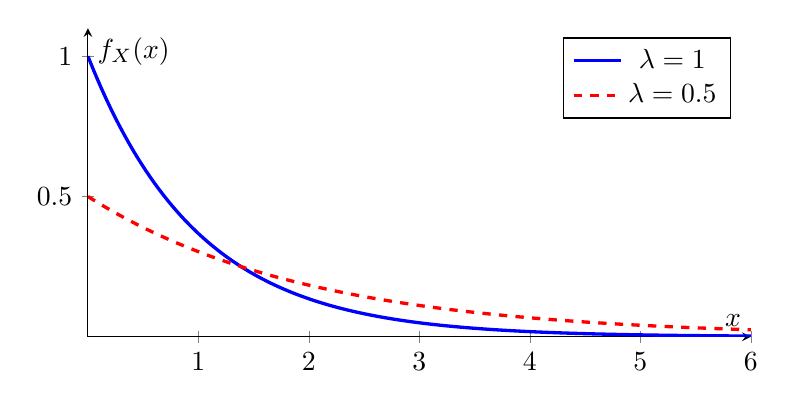
\begin{tikzpicture}
\begin{axis}[
    width=10cm,
    height=5.5cm,
    axis lines=middle,
    xlabel={$x$},
    ylabel={$f_X(x)$},
    xmin=0,
    xmax=6,
    ymin=0,
    ymax=1.1,
    samples=150,
    domain=0:6,
    legend pos=north east
]
\addplot[blue,very thick]{exp(-x)};
\addlegendentry{$\lambda=1$}

\addplot[red,very thick,dashed]
{0.5*exp(-0.5*x)};
\addlegendentry{$\lambda=0.5$}
\end{axis}
\end{tikzpicture}
\end{center}

All'aumentare di $\lambda$,
il tempo medio di attesa diminuisce.

\begin{example}{Tempo di attesa di un server}

Supponiamo che il tempo tra
due richieste consecutive
segua una distribuzione esponenziale
con
\[
\lambda=0.5\text{ richieste/secondo}.
\]

Il tempo medio di attesa è
\[
\mathbb{E}[X]=\frac1{0.5}=2\text{ s}.
\]

Vogliamo calcolare
la probabilità di attendere
più di 3 secondi:
\[
P(X>3)=e^{-0.5\cdot3}.
\]

Quindi:
\[
\boxed{
P(X>3)=e^{-1.5}\approx0.2231.
}
\]

La probabilità è circa il $22.31\%$.
\end{example}


\subsection{Distribuzione normale o gaussiana}

\subsubsection{Idea intuitiva}

La distribuzione normale
è una delle distribuzioni
più importanti della probabilità
e della statistica.

È caratterizzata da una curva
a forma di campana,
simmetrica rispetto alla media.

Compare frequentemente
in modelli approssimativi di:
\begin{itemize}
    \item errori di misurazione;
    \item caratteristiche biologiche;
    \item rumore in segnali;
    \item somme di molti piccoli
    contributi casuali.
\end{itemize}

Un ruolo importante è svolto
dal teorema centrale del limite.

\begin{definition}{Distribuzione normale}
Una variabile aleatoria $X$
segue una distribuzione normale
con parametri $\mu\in\mathbb{R}$
e $\sigma^2>0$ se
\[
\boxed{
f_X(x)
=
\frac1{\sigma\sqrt{2\pi}}
\exp\left(
-\frac{(x-\mu)^2}{2\sigma^2}
\right),
\qquad x\in\mathbb{R}.
}
\]

Si scrive
\[
X\sim\mathcal{N}(\mu,\sigma^2).
\]
\end{definition}

I parametri sono:
\[
\mu=\mathbb{E}[X],
\]
\[
\sigma^2=\operatorname{Var}(X).
\]

\subsubsection{Ruolo dei parametri}

\paragraph{Parametro $\mu$}

Determina la posizione
del centro della distribuzione.

Se $\mu$ aumenta,
la curva si sposta verso destra.

\paragraph{Parametro $\sigma$}

Determina la dispersione.

Un valore piccolo di $\sigma$
produce una curva più concentrata.

Un valore grande di $\sigma$
produce una curva più larga
e con un picco meno elevato.

\subsubsection{Grafico della distribuzione normale}

\begin{center}
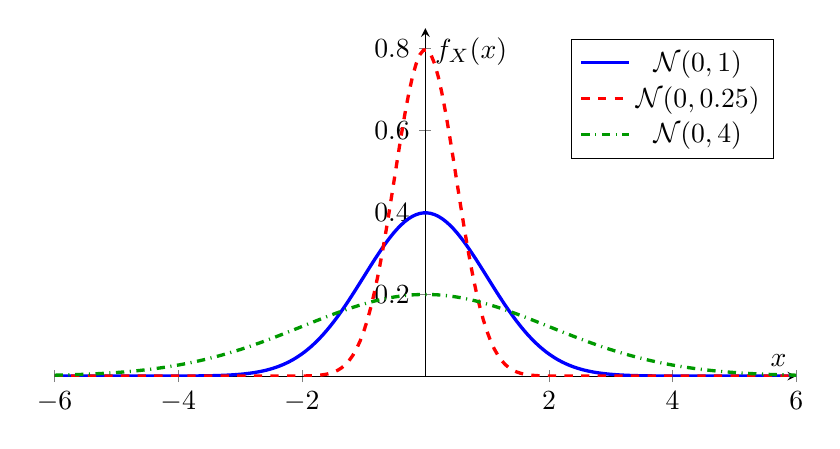
\begin{tikzpicture}
\begin{axis}[
    width=11cm,
    height=6cm,
    xlabel={$x$},
    ylabel={$f_X(x)$},
    xmin=-6,
    xmax=6,
    ymin=0,
    ymax=0.85,
    axis lines=middle,
    samples=200,
    domain=-6:6,
    legend pos=north east
]
\addplot[blue,very thick]
{exp(-x^2/2)/sqrt(2*pi)};
\addlegendentry{$\mathcal{N}(0,1)$}

\addplot[red,dashed,very thick]
{exp(-x^2/(2*0.5^2))/(0.5*sqrt(2*pi))};
\addlegendentry{$\mathcal{N}(0,0.25)$}

\addplot[green!60!black,dashdotted,very thick]
{exp(-x^2/(2*2^2))/(2*sqrt(2*pi))};
\addlegendentry{$\mathcal{N}(0,4)$}
\end{axis}
\end{tikzpicture}
\end{center}

Le tre distribuzioni hanno
la stessa media, ma varianze diverse.

\subsubsection{Proprietà principali}

\paragraph{Simmetria}

La densità è simmetrica
rispetto a $\mu$:
\[
f_X(\mu-t)=f_X(\mu+t).
\]

\paragraph{Coincidenza tra media, mediana e moda}

\[
\boxed{
\text{Media}=\text{Mediana}=\text{Moda}=\mu.
}
\]

\paragraph{Supporto}

\[
\operatorname{supp}(X)=\mathbb{R}.
\]

\paragraph{Trasformazioni affini}

Se
\[
X\sim\mathcal{N}(\mu,\sigma^2),
\]
allora, per $a\neq0$:
\[
aX+b
\sim
\mathcal{N}(a\mu+b,a^2\sigma^2).
\]

\subsubsection{Distribuzione normale standard}

\begin{definition}{Normale standard}
La distribuzione normale standard
è la normale con media 0
e varianza 1:
\[
\boxed{
Z\sim\mathcal{N}(0,1).
}
\]

La sua densità è:
\[
\boxed{
\varphi(z)
=
\frac1{\sqrt{2\pi}}e^{-z^2/2}.
}
\]
\end{definition}

La funzione di ripartizione
della normale standard è
\[
\boxed{
\Phi(z)
=
\int_{-\infty}^{z}
\frac1{\sqrt{2\pi}}e^{-t^2/2}\,dt.
}
\]

Tale integrale non possiede
una primitiva esprimibile
mediante le funzioni elementari.

Per questo motivo,
le probabilità vengono generalmente
calcolate mediante tabelle,
software o metodi numerici.

\subsubsection{Standardizzazione}

Se
\[
X\sim\mathcal{N}(\mu,\sigma^2),
\]
possiamo definire
\[
\boxed{
Z=\frac{X-\mu}{\sigma}.
}
\]

Allora:
\[
\boxed{
Z\sim\mathcal{N}(0,1).
}
\]

Di conseguenza:
\[
P(X\leq x)
=
\Phi\left(\frac{x-\mu}{\sigma}\right).
\]

\begin{example}{Calcolo di una probabilità normale}

Supponiamo che il peso
di un componente prodotto
industrialmente segua:
\[
X\sim\mathcal{N}(100,16).
\]

Quindi:
\[
\mu=100,
\qquad
\sigma=4.
\]

Vogliamo determinare
\[
P(X\leq104).
\]

Standardizziamo:
\[
Z=\frac{X-100}{4}.
\]

Quindi:
\[
P(X\leq104)
=
P\left(
Z\leq\frac{104-100}{4}
\right).
\]

Otteniamo:
\[
=P(Z\leq1)=\Phi(1).
\]

Utilizzando una tabella
della normale standard:
\[
\Phi(1)\approx0.8413.
\]

Pertanto:
\[
\boxed{
P(X\leq104)\approx0.8413.
}
\]

Circa l'84.13\% dei componenti
ha un peso non superiore a 104.
\end{example}

\subsubsection{Regola empirica 68--95--99.7}

Per una variabile normale:
\[
P(\mu-\sigma\leq X\leq\mu+\sigma)
\approx0.6827,
\]

\[
P(\mu-2\sigma\leq X\leq\mu+2\sigma)
\approx0.9545,
\]

\[
P(\mu-3\sigma\leq X\leq\mu+3\sigma)
\approx0.9973.
\]

Questa regola permette
di interpretare rapidamente
la concentrazione dei valori
attorno alla media.


\subsection{Distribuzione Gamma}

\subsubsection{Idea intuitiva}

La distribuzione Gamma
generalizza la distribuzione esponenziale.

È particolarmente utile
per modellare tempi di attesa
fino al verificarsi
di un certo numero di eventi
in un processo di Poisson.

\begin{definition}{Distribuzione Gamma}
Una variabile aleatoria $X$
segue una distribuzione Gamma
con parametri di forma
$\alpha>0$ e tasso $\lambda>0$ se
\[
\boxed{
f_X(x)
=
\begin{cases}
\frac{\lambda^\alpha}{\Gamma(\alpha)}
x^{\alpha-1}e^{-\lambda x}
& x>0,\\
0 & x\leq0.
\end{cases}
}
\]

Si scrive
\[
X\sim\operatorname{Gamma}(\alpha,\lambda).
\]
\end{definition}

La funzione Gamma è definita da
\[
\boxed{
\Gamma(\alpha)
=
\int_0^\infty t^{\alpha-1}e^{-t}\,dt.
}
\]

Per interi positivi $n$:
\[
\Gamma(n)=(n-1)!.
\]

\subsubsection{Media e varianza}

Nella parametrizzazione
con il tasso $\lambda$:
\[
\boxed{
\mathbb{E}[X]=\frac{\alpha}{\lambda}.
}
\]

\[
\boxed{
\operatorname{Var}(X)=\frac{\alpha}{\lambda^2}.
}
\]

\subsubsection{Legame con la distribuzione esponenziale}

Se $\alpha=1$, allora:
\[
\Gamma(1)=1.
\]

La densità diventa:
\[
f_X(x)=\lambda e^{-\lambda x}.
\]

Quindi:
\[
\boxed{
\operatorname{Gamma}(1,\lambda)
=
\operatorname{Exp}(\lambda).
}
\]

\begin{example}{Attesa della terza richiesta}

Supponiamo che le richieste
arrivino a un server
secondo un processo di Poisson
con tasso
\[
\lambda=2
\quad\text{richieste/minuto}.
\]

Indichiamo con $X$
il tempo fino alla terza richiesta.

Allora:
\[
X\sim\operatorname{Gamma}(3,2).
\]

Il tempo medio è:
\[
\mathbb{E}[X]=\frac32=1.5
\text{ minuti}.
\]

La varianza è:
\[
\operatorname{Var}(X)
=
\frac3{2^2}
=
\frac34
\text{ minuti}^2.
\]
\end{example}


\subsection{Distribuzione Beta}

\subsubsection{Idea intuitiva}

La distribuzione Beta
è definita nell'intervallo $[0,1]$.

È particolarmente adatta
per modellare quantità
che rappresentano:
\begin{itemize}
    \item proporzioni;
    \item percentuali normalizzate;
    \item probabilità sconosciute;
    \item frazioni di una quantità totale.
\end{itemize}

\begin{definition}{Distribuzione Beta}
Una variabile aleatoria $X$
segue una distribuzione Beta
di parametri $\alpha,\beta>0$
se:
\[
\boxed{
f_X(x)=
\begin{cases}
\frac{x^{\alpha-1}(1-x)^{\beta-1}}
{B(\alpha,\beta)}
& 0<x<1,\\
0 & \text{altrimenti}.
\end{cases}
}
\]

Si scrive
\[
X\sim\operatorname{Beta}(\alpha,\beta).
\]
\end{definition}

La funzione Beta è:
\[
B(\alpha,\beta)
=
\int_0^1
x^{\alpha-1}(1-x)^{\beta-1}\,dx.
\]

È legata alla funzione Gamma:
\[
\boxed{
B(\alpha,\beta)
=
\frac{\Gamma(\alpha)\Gamma(\beta)}
{\Gamma(\alpha+\beta)}.
}
\]

\subsubsection{Media e varianza}

\[
\boxed{
\mathbb{E}[X]
=
\frac{\alpha}{\alpha+\beta}.
}
\]

\[
\boxed{
\operatorname{Var}(X)
=
\frac{\alpha\beta}
{(\alpha+\beta)^2(\alpha+\beta+1)}.
}
\]

\subsubsection{Interpretazione dei parametri}

La distribuzione Beta
può assumere forme differenti.

\begin{itemize}
    \item $\alpha=\beta=1$:
    distribuzione uniforme su $[0,1]$.

    \item $\alpha>\beta$:
    maggiore concentrazione
    verso valori elevati,
    in termini di media.

    \item $\alpha<\beta$:
    maggiore concentrazione
    verso valori bassi.

    \item $\alpha,\beta>1$:
    densità con un massimo interno.
\end{itemize}

\begin{example}{Modellazione di una probabilità}

Supponiamo di voler rappresentare
l'incertezza su una probabilità
di successo $p$.

Possiamo modellare $p$ mediante
\[
p\sim\operatorname{Beta}(8,2).
\]

La media è
\[
\mathbb{E}[p]
=
\frac8{8+2}
=
0.8.
\]

Questo significa che,
secondo la distribuzione scelta,
il valore medio della probabilità
incognita è $0.8$.

La distribuzione Beta è molto
utilizzata nella statistica bayesiana
come distribuzione a priori
per il parametro di Bernoulli.
\end{example}


\subsection{Distribuzione chi-quadrato}

\subsubsection{Idea intuitiva}

La distribuzione chi-quadrato
compare soprattutto
in statistica inferenziale.

Nasce dalla somma dei quadrati
di variabili normali standard indipendenti.

\begin{definition}{Distribuzione chi-quadrato}
Siano
\[
Z_1,\ldots,Z_k
\]
variabili aleatorie indipendenti,
ciascuna distribuita come
$\mathcal{N}(0,1)$.

La variabile
\[
\boxed{
X=\sum_{i=1}^{k}Z_i^2
}
\]
segue una distribuzione
chi-quadrato con $k$
gradi di libertà.

Si scrive
\[
X\sim\chi_k^2.
\]
\end{definition}

La densità è:
\[
f_X(x)
=
\frac{1}{2^{k/2}\Gamma(k/2)}
x^{k/2-1}e^{-x/2},
\qquad x>0.
\]

\subsubsection{Media e varianza}

\[
\boxed{
\mathbb{E}[X]=k.
}
\]

\[
\boxed{
\operatorname{Var}(X)=2k.
}
\]

\subsubsection{Relazione con la Gamma}

\[
\boxed{
\chi_k^2
=
\operatorname{Gamma}\left(\frac{k}{2},\frac12\right)
}
\]

nella parametrizzazione Gamma
che utilizza il tasso.

\paragraph{Applicazioni}

La distribuzione chi-quadrato
è utilizzata, tra le altre cose,
nei test di adattamento,
nei test d'indipendenza
e nell'inferenza sulla varianza
di popolazioni normali.


\subsection{Distribuzione t di Student}

\subsubsection{Idea intuitiva}

La distribuzione t di Student
è simmetrica e simile
alla distribuzione normale,
ma possiede code più pesanti.

È importante quando
si fanno inferenze sulla media
di una popolazione normale
e la varianza è sconosciuta.

\begin{definition}{Distribuzione t di Student}
Siano
\[
Z\sim\mathcal{N}(0,1)
\]
e
\[
V\sim\chi_\nu^2
\]
indipendenti.

Allora:
\[
\boxed{
T=\frac{Z}{\sqrt{V/\nu}}
}
\]
segue una distribuzione
t di Student con $\nu$
gradi di libertà.

Si scrive
\[
T\sim t_\nu.
\]
\end{definition}

La densità è:
\[
f_T(t)
=
\frac{\Gamma((\nu+1)/2)}
{\sqrt{\nu\pi}\Gamma(\nu/2)}
\left(1+\frac{t^2}{\nu}\right)^{-(\nu+1)/2}.
\]

\subsubsection{Media e varianza}

Per $\nu>1$:
\[
\mathbb{E}[T]=0.
\]

Per $\nu>2$:
\[
\operatorname{Var}(T)=\frac{\nu}{\nu-2}.
\]

Per $\nu\leq1$ la media
non esiste; per
$1<\nu\leq2$ la varianza
non è finita.

\paragraph{Proprietà asintotica}

Al crescere dei gradi di libertà:
\[
t_\nu
\xrightarrow{d}
\mathcal{N}(0,1).
\]

La distribuzione t
si avvicina quindi
alla normale standard.


\subsection{Distribuzione F di Fisher--Snedecor}

\subsubsection{Idea intuitiva}

La distribuzione F
è utilizzata soprattutto
per confrontare varianze
e nell'analisi della varianza (ANOVA).

\begin{definition}{Distribuzione F}
Siano
\[
U\sim\chi_{d_1}^2,
\qquad
V\sim\chi_{d_2}^2
\]
indipendenti.

La variabile
\[
\boxed{
F=\frac{U/d_1}{V/d_2}
}
\]
segue una distribuzione F
con $d_1$ e $d_2$
gradi di libertà.

Si scrive
\[
F\sim F_{d_1,d_2}.
\]
\end{definition}

La distribuzione è definita
per valori positivi.

\subsubsection{Media e varianza}

Se $d_2>2$:
\[
\boxed{
\mathbb{E}[F]=\frac{d_2}{d_2-2}.
}
\]

Se $d_2>4$:
\[
\boxed{
\operatorname{Var}(F)
=
\frac{2d_2^2(d_1+d_2-2)}
{d_1(d_2-2)^2(d_2-4)}.
}
\]

Per $d_2\leq2$ la media
non è finita; per
$2<d_2\leq4$ la varianza
non è finita.


\section{Trasformazioni di Variabili Aleatorie Continue}

\subsection{Trasformazione affine}

Supponiamo di definire
una nuova variabile aleatoria
\[
Y=aX+b,
\qquad a\neq0.
\]

Allora:
\[
\boxed{
\mathbb{E}[Y]
=
a\mathbb{E}[X]+b.
}
\]

\[
\boxed{
\operatorname{Var}(Y)
=
a^2\operatorname{Var}(X).
}
\]

Se $X$ ha densità $f_X$,
la densità di $Y$ è
\[
\boxed{
f_Y(y)
=
\frac1{|a|}
f_X\left(\frac{y-b}{a}\right).
}
\]

\begin{example}{Conversione di temperatura}

Sia $X$ una temperatura
casuale espressa in gradi Celsius.

Definiamo la temperatura
in gradi Fahrenheit:
\[
Y=\frac95 X+32.
\]

Se
\[
\mathbb{E}[X]=20,
\]
allora
\[
\mathbb{E}[Y]
=
\frac95\cdot20+32
=
68.
\]

Se
\[
\operatorname{Var}(X)=4,
\]
allora
\[
\operatorname{Var}(Y)
=
\left(\frac95\right)^2\cdot4
=
12.96.
\]
\end{example}

\subsection{Trasformazione monotona}

Sia
\[
Y=g(X),
\]
dove $g$ è strettamente monotona,
derivabile e dotata
di inversa derivabile
sull'intervallo considerato.

Allora:
\[
\boxed{
f_Y(y)
=
f_X(g^{-1}(y))
\left|
\frac{d}{dy}g^{-1}(y)
\right|.
}
\]

Questa formula permette
di ottenere la densità
di una variabile trasformata.

\begin{example}{Trasformazione quadratica}

Sia
\[
X\sim\mathcal{U}(0,1)
\]
e definiamo
\[
Y=X^2.
\]

Poiché $X\in[0,1]$,
la funzione $g(x)=x^2$
è strettamente crescente.

L'inversa è
\[
x=\sqrt y.
\]

La derivata è:
\[
\frac{dx}{dy}
=
\frac1{2\sqrt y}.
\]

Dato che
\[
f_X(x)=1
\quad\text{per }0<x<1,
\]
otteniamo:
\[
\boxed{
f_Y(y)=
\begin{cases}
\frac1{2\sqrt y} & 0<y<1,\\
0 & \text{altrimenti}.
\end{cases}
}
\]

Verifichiamo:
\[
\int_0^1
\frac1{2\sqrt y}\,dy
=
[\sqrt y]_0^1
=
1.
\]
\end{example}

\paragraph{Trasformazioni non monotone}

Se la trasformazione $g$
non è iniettiva, sotto opportune
condizioni di regolarità
si devono sommare
i contributi delle diverse
soluzioni di $g(x)=y$:

\[
f_Y(y)
=
\sum_{x_i:g(x_i)=y}
\frac{f_X(x_i)}{|g'(x_i)|}.
\]

La formula vale nei punti
per i quali le preimmagini
sono regolari e le derivate
al denominatore sono non nulle.


\section{Variabili Aleatorie Continue Congiunte}

\subsection{Densità congiunta}

Quando studiamo due variabili
aleatorie contemporaneamente,
non basta conoscere separatamente
le loro distribuzioni.

È necessario descrivere
anche la dipendenza
tra le due variabili.

\begin{definition}{Densità congiunta}
Due variabili aleatorie $X,Y$
sono congiuntamente assolutamente continue
se esiste una funzione
\[
f_{X,Y}(x,y)\geq0
\]
tale che, per ogni insieme
boreliano $A\subseteq\mathbb{R}^2$:
\[
\boxed{
P((X,Y)\in A)
=
\iint_A f_{X,Y}(x,y)\,dx\,dy.
}
\]
\end{definition}

La densità congiunta deve soddisfare:
\[
\boxed{
\int_{-\infty}^{+\infty}
\int_{-\infty}^{+\infty}
f_{X,Y}(x,y)\,dy\,dx
=
1.
}
\]

\subsection{Densità marginali}

Le densità marginali
si ottengono integrando
la densità congiunta
rispetto all'altra variabile.

\[
\boxed{
f_X(x)
=
\int_{-\infty}^{+\infty}
f_{X,Y}(x,y)\,dy.
}
\]

\[
\boxed{
f_Y(y)
=
\int_{-\infty}^{+\infty}
f_{X,Y}(x,y)\,dx.
}
\]

\subsection{Indipendenza}

\begin{definition}{Indipendenza}
Due variabili aleatorie
congiuntamente assolutamente continue
$X$ e $Y$ sono indipendenti
se e solo se:
\[
\boxed{
f_{X,Y}(x,y)=f_X(x)f_Y(y)
}
\]
quasi ovunque.
\end{definition}

\subsection{Densità condizionata}

Per un valore $x$ tale che
$f_X(x)>0$:
\[
\boxed{
f_{Y\mid X}(y\mid x)
=
\frac{f_{X,Y}(x,y)}{f_X(x)}.
}
\]

La funzione rappresenta
la densità condizionata di $Y$
dato il valore $X=x$.

L'interpretazione è importante:
anche se in una distribuzione continua
\[
P(X=x)=0,
\]
è possibile definire
rigorosamente distribuzioni condizionate
tramite densità e probabilità
condizionate regolari.


\subsection{Covarianza e correlazione}

\begin{definition}{Covarianza}
Per due variabili aleatorie
con secondi momenti finiti,
la covarianza è:
\[
\boxed{
\operatorname{Cov}(X,Y)
=
\mathbb{E}[
(X-\mathbb{E}[X])
(Y-\mathbb{E}[Y])
].
}
\]
\end{definition}

La formula equivalente è:
\[
\boxed{
\operatorname{Cov}(X,Y)
=
\mathbb{E}[XY]
-
\mathbb{E}[X]\mathbb{E}[Y].
}
\]

Nel caso congiuntamente continuo:
\[
\mathbb{E}[XY]
=
\int_{-\infty}^{+\infty}
\int_{-\infty}^{+\infty}
xyf_{X,Y}(x,y)\,dy\,dx.
\]

\begin{definition}{Coefficiente di correlazione}
Se le deviazioni standard
sono finite e positive:
\[
\boxed{
\rho_{X,Y}
=
\frac{\operatorname{Cov}(X,Y)}
{\sigma_X\sigma_Y}.
}
\]
\end{definition}

Si ha:
\[
-1\leq\rho_{X,Y}\leq1.
\]

\begin{itemize}
    \item $\rho>0$: associazione lineare positiva.
    \item $\rho<0$: associazione lineare negativa.
    \item $\rho=0$: assenza di correlazione lineare.
\end{itemize}

L'indipendenza implica
covarianza nulla, quando
i momenti necessari esistono.

Il viceversa, in generale,
non è vero.


\section{Teorema Centrale del Limite}

Il teorema centrale del limite
spiega una delle ragioni
per cui la distribuzione normale
è così importante.

\begin{theorem}{Teorema centrale del limite}
Siano
\[
X_1,X_2,\ldots
\]
variabili aleatorie indipendenti
e identicamente distribuite,
con
\[
\mathbb{E}[X_i]=\mu
\]
e
\[
0<\operatorname{Var}(X_i)=\sigma^2<+\infty.
\]

Definiamo la media campionaria:
\[
\overline X_n
=
\frac1n\sum_{i=1}^{n}X_i.
\]

Allora:
\[
\boxed{
\frac{\sqrt n(\overline X_n-\mu)}{\sigma}
\xrightarrow{d}
\mathcal{N}(0,1)
}
\]
quando $n\to+\infty$.
\end{theorem}

\paragraph{Interpretazione}

Se prendiamo molte osservazioni
indipendenti della stessa distribuzione
e ne calcoliamo la media,
la distribuzione della media
standardizzata tende
a una normale standard,
anche quando le osservazioni
originali non sono normalmente distribuite.

Per un numero di osservazioni
sufficientemente grande,
in condizioni in cui
l'approssimazione è adeguata:
\[
\boxed{
\overline X_n
\approx
\mathcal{N}
\left(\mu,\frac{\sigma^2}{n}\right).
}
\]

Il valore di $n$ necessario
per ottenere una buona approssimazione
dipende dalla distribuzione di partenza.

\begin{example}{Media dei tempi di risposta}

Supponiamo che il tempo di risposta
di un sistema abbia:
\[
\mathbb{E}[X]=10\text{ ms}
\]
e
\[
\operatorname{Var}(X)=16\text{ ms}^2.
\]

Consideriamo la media
di $n=100$ osservazioni
indipendenti e identicamente distribuite.

La media campionaria ha:
\[
\mathbb{E}[\overline X_{100}]=10.
\]

La sua varianza è:
\[
\operatorname{Var}(\overline X_{100})
=
\frac{16}{100}=0.16.
\]

La deviazione standard
della media campionaria è:
\[
\sigma_{\overline X}
=
\sqrt{0.16}=0.4\text{ ms}.
\]

Per il teorema centrale del limite:
\[
\overline X_{100}
\approx
\mathcal{N}(10,0.16).
\]

L'approssimazione permette
di stimare probabilità
relative alla media campionaria.
\end{example}


\section{Confronto tra Distribuzioni Discrete e Continue}

\begin{center}
\renewcommand{\arraystretch}{1.5}
\begin{tabular}{|p{4cm}|p{4.5cm}|p{4.5cm}|}
\hline
\textbf{Caratteristica}
&
\textbf{Discreta}
&
\textbf{Assolutamente continua}
\\
\hline
Descrizione
&
Funzione di massa (PMF)
&
Funzione di densità (PDF)
\\
\hline
Probabilità puntuale
&
$P(X=x)$ può essere positiva
&
$P(X=x)=0$
\\
\hline
Probabilità di intervalli
&
Somma delle masse
&
Integrale della densità
\\
\hline
Normalizzazione
&
$\sum_x p_X(x)=1$
&
$\int_{\mathbb R}f_X(x)\,dx=1$
\\
\hline
Valore atteso
&
$\sum_x xp_X(x)$
&
$\int_{\mathbb R}xf_X(x)\,dx$
\\
\hline
Varianza
&
$\sum_x(x-\mu)^2p_X(x)$
&
$\int_{\mathbb R}(x-\mu)^2f_X(x)\,dx$
\\
\hline
\end{tabular}
\end{center}


\section{Tabella Riassuntiva delle Principali Distribuzioni}

\begin{center}
\renewcommand{\arraystretch}{1.6}
\small
\begin{tabular}{|p{3.2cm}|p{3.4cm}|p{3.5cm}|p{3.5cm}|}
\hline
\textbf{Distribuzione}
&
\textbf{Supporto}
&
\textbf{Media}
&
\textbf{Varianza}
\\
\hline
Uniforme $\mathcal U(a,b)$
&
$[a,b]$
&
$\frac{a+b}{2}$
&
$\frac{(b-a)^2}{12}$
\\
\hline
Esponenziale $\operatorname{Exp}(\lambda)$
&
$[0,+\infty)$
&
$\frac1\lambda$
&
$\frac1{\lambda^2}$
\\
\hline
Normale $\mathcal N(\mu,\sigma^2)$
&
$\mathbb R$
&
$\mu$
&
$\sigma^2$
\\
\hline
Gamma $(\alpha,\lambda)$
&
$[0,+\infty)$
&
$\frac{\alpha}{\lambda}$
&
$\frac{\alpha}{\lambda^2}$
\\
\hline
Beta $(\alpha,\beta)$
&
$[0,1]$
&
$\frac{\alpha}{\alpha+\beta}$
&
$\frac{\alpha\beta}
{(\alpha+\beta)^2(\alpha+\beta+1)}$
\\
\hline
Chi-quadrato $\chi_k^2$
&
$[0,+\infty)$
&
$k$
&
$2k$
\\
\hline
Student $t_\nu$
&
$\mathbb R$
&
$0$, se $\nu>1$
&
$\frac{\nu}{\nu-2}$, se $\nu>2$
\\
\hline
Fisher $F_{d_1,d_2}$
&
$[0,+\infty)$
&
$\frac{d_2}{d_2-2}$, se $d_2>2$
&
$\frac{2d_2^2(d_1+d_2-2)}
{d_1(d_2-2)^2(d_2-4)}$,
se $d_2>4$
\\
\hline
\end{tabular}
\end{center}


\section{Schema Operativo per Risolvere gli Esercizi}

Quando viene assegnata una variabile aleatoria
continua attraverso una densità $f_X(x)$,
si può seguire il procedimento seguente.

\subsection*{1. Verificare che sia una densità}

Controllare:
\[
f_X(x)\geq0
\]
e
\[
\int_{-\infty}^{+\infty}f_X(x)\,dx=1.
\]

\subsection*{2. Identificare il supporto}

Individuare la regione
in cui è concentrata
la probabilità.

\subsection*{3. Calcolare la CDF}

\[
F_X(x)
=
\int_{-\infty}^{x}f_X(t)\,dt.
\]

Prestare attenzione agli intervalli
in cui la densità è nulla.

\subsection*{4. Calcolare le probabilità}

Utilizzare:
\[
P(a\leq X\leq b)
=
\int_a^b f_X(x)\,dx
\]
oppure:
\[
P(a\leq X\leq b)
=
F_X(b)-F_X(a).
\]

\subsection*{5. Calcolare la media}

\[
\mu
=
\int_{-\infty}^{+\infty}
xf_X(x)\,dx.
\]

\subsection*{6. Calcolare il secondo momento}

\[
\mathbb{E}[X^2]
=
\int_{-\infty}^{+\infty}
x^2f_X(x)\,dx.
\]

\subsection*{7. Calcolare la varianza}

\[
\operatorname{Var}(X)
=
\mathbb{E}[X^2]-\mu^2.
\]

\subsection*{8. Calcolare la deviazione standard}

\[
\sigma_X
=
\sqrt{\operatorname{Var}(X)}.
\]


\section{Esercizio Riepilogativo Completo}

\begin{example}{Studio completo di una densità}

Sia $X$ una variabile aleatoria continua
con densità:
\[
f_X(x)=
\begin{cases}
cx^2 & 0\leq x\leq2,\\
0 & \text{altrove}.
\end{cases}
\]

Determinare:
\begin{enumerate}
    \item il valore della costante $c$;
    \item la funzione di ripartizione;
    \item la probabilità $P(1\leq X\leq2)$;
    \item il valore atteso;
    \item la varianza;
    \item la deviazione standard.
\end{enumerate}

\textbf{1. Determinazione della costante.}

Dalla normalizzazione:
\[
\int_0^2 cx^2\,dx=1.
\]

Portiamo fuori $c$:
\[
c\int_0^2x^2\,dx=1.
\]

\[
c\left[\frac{x^3}{3}\right]_0^2=1.
\]

Quindi:
\[
c\frac83=1.
\]

Otteniamo:
\[
\boxed{c=\frac38}.
\]

La densità è:
\[
f_X(x)=
\begin{cases}
\frac38x^2 & 0\leq x\leq2,\\
0 & \text{altrove}.
\end{cases}
\]

\textbf{2. Calcolo della CDF.}

Per $x<0$:
\[
F_X(x)=0.
\]

Per $0\leq x\leq2$:
\[
F_X(x)
=
\int_0^x\frac38t^2\,dt.
\]

\[
=
\frac38
\left[\frac{t^3}{3}\right]_0^x.
\]

Quindi:
\[
F_X(x)=\frac{x^3}{8}.
\]

Per $x>2$:
\[
F_X(x)=1.
\]

Pertanto:
\[
\boxed{
F_X(x)=
\begin{cases}
0 & x<0,\\
\frac{x^3}{8} & 0\leq x\leq2,\\
1 & x>2.
\end{cases}
}
\]

\textbf{3. Calcolo della probabilità.}

\[
P(1\leq X\leq2)
=
F_X(2)-F_X(1).
\]

\[
=
1-\frac18.
\]

Quindi:
\[
\boxed{
P(1\leq X\leq2)=\frac78.
}
\]

\textbf{4. Calcolo della media.}

\[
\mathbb{E}[X]
=
\int_0^2 x\frac38x^2\,dx.
\]

\[
=
\frac38\int_0^2x^3\,dx.
\]

\[
=
\frac38
\left[\frac{x^4}{4}\right]_0^2.
\]

\[
=
\frac38\cdot4.
\]

Quindi:
\[
\boxed{
\mathbb{E}[X]=\frac32.
}
\]

\textbf{5. Calcolo del secondo momento.}

\[
\mathbb{E}[X^2]
=
\int_0^2x^2\frac38x^2\,dx.
\]

\[
=
\frac38\int_0^2x^4\,dx.
\]

\[
=
\frac38
\left[\frac{x^5}{5}\right]_0^2.
\]

\[
=
\frac38\cdot\frac{32}{5}.
\]

Quindi:
\[
\boxed{
\mathbb{E}[X^2]=\frac{12}{5}.
}
\]

\textbf{6. Calcolo della varianza.}

\[
\operatorname{Var}(X)
=
\frac{12}{5}
-
\left(\frac32\right)^2.
\]

\[
=
\frac{12}{5}-\frac94.
\]

\[
=
\frac{48}{20}-\frac{45}{20}.
\]

Pertanto:
\[
\boxed{
\operatorname{Var}(X)=\frac3{20}.
}
\]

\textbf{7. Calcolo della deviazione standard.}

\[
\sigma_X
=
\sqrt{\frac3{20}}.
\]

Quindi:
\[
\boxed{
\sigma_X\approx0.3873.
}
\]

\paragraph{Interpretazione finale}

La variabile aleatoria $X$
assume valori nell'intervallo $[0,2]$.

La densità cresce
proporzionalmente a $x^2$,
quindi la probabilità
è maggiormente concentrata
verso la parte destra
dell'intervallo.

Questo spiega perché
il valore atteso
\[
\mathbb{E}[X]=1.5
\]
è maggiore del punto medio
dell'intervallo, pari a 1.
\end{example}
